\documentclass[tikz,border=10pt]{standalone}
\begin{document}
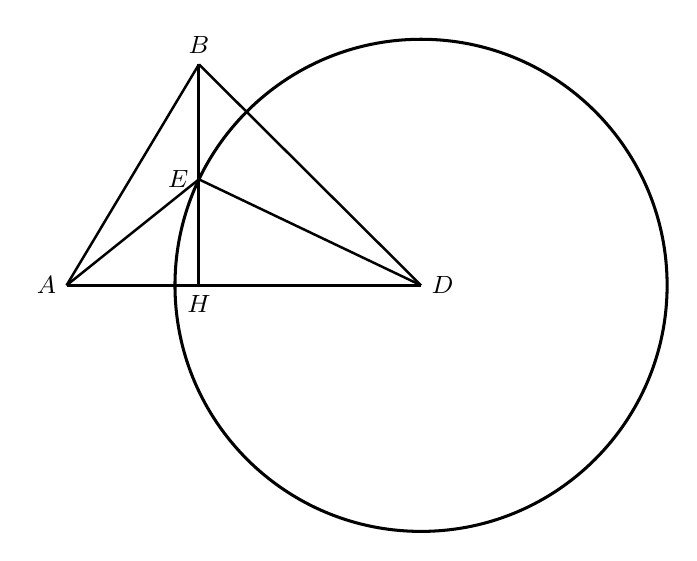
\begin{tikzpicture}[line width=0.9pt, line join=round]
% Points: s = 0.01194 cm/px, centre (385,312.5) px
\coordinate (A) at (-3.651,0);
\coordinate (B) at (-1.970,2.806);
\coordinate (E) at (-1.970,1.346);
\coordinate (H) at (-1.970,0);
\coordinate (D) at (0.851,0);

% Circle centred at D, radius 262 px (heavier weight to match original)
\draw[line width=1.1pt] (D) circle[radius=3.125];

% Solid segments (AD and BH at 1.1pt to match original weight)
\draw[line width=1.1pt] (A) -- (D);
\draw (A) -- (B);
\draw[line width=1.1pt] (B) -- (H);
\draw (A) -- (E);
\draw (E) -- (D);
\draw (B) -- (D);

% Labels (9.5 pt font from style metrics); H placed directly below its point
\node[above, font=\fontsize{9.5}{11.4}\selectfont] at (B) {$B$};
\node[left, font=\fontsize{9.5}{11.4}\selectfont] at (E) {$E$};
\node[left, font=\fontsize{9.5}{11.4}\selectfont] at (A) {$A$};
\node[right, font=\fontsize{9.5}{11.4}\selectfont] at (D) {$D$};
\node[below, font=\fontsize{9.5}{11.4}\selectfont] at (H) {$H$};
\end{tikzpicture}
\end{document}